% THIS DOCUMENT IS FOLLOWS THE VOLERE TEMPLATE BY Suzanne Robertson and James Robertson
% ONLY THE SECTION HEADINGS ARE PROVIDED
%
% Initial draft from https://github.com/Dieblich/volere
%
% Risks are removed because they are covered by the Hazard Analysis
\documentclass[12pt]{article}

\usepackage{booktabs}
\usepackage{tabularx}
\usepackage{graphicx}
\usepackage{float}
\usepackage{hyperref}
\hypersetup{
    bookmarks=true,         % show bookmarks bar?
      colorlinks=true,      % false: boxed links; true: colored links
    linkcolor=red,          % color of internal links (change box color with linkbordercolor)
    citecolor=green,        % color of links to bibliography
    filecolor=magenta,      % color of file links
    urlcolor=cyan           % color of external links
}

\newcommand{\lips}{\textit{Insert your content here.}}

%% Comments

\usepackage{color}

\newif\ifcomments\commentstrue %displays comments
%\newif\ifcomments\commentsfalse %so that comments do not display

\ifcomments
\newcommand{\authornote}[3]{\textcolor{#1}{[#3 ---#2]}}
\newcommand{\todo}[1]{\textcolor{red}{[TODO: #1]}}
\else
\newcommand{\authornote}[3]{}
\newcommand{\todo}[1]{}
\fi

\newcommand{\wss}[1]{\authornote{blue}{SS}{#1}} 
\newcommand{\plt}[1]{\authornote{magenta}{TPLT}{#1}} %For explanation of the template
\newcommand{\an}[1]{\authornote{cyan}{Author}{#1}}

%% Common Parts

\newcommand{\progname}{Software Engineering}
\newcommand{\authname}{Team 1, BANDwidth
\\ Declan Young
\\ Ben Dubois
\\ Nathan Uy
\\ Aidan Mariglia}                

\usepackage{hyperref}
    \hypersetup{colorlinks=true, linkcolor=blue, citecolor=blue, filecolor=blue,
                urlcolor=blue, unicode=false}
    \urlstyle{same}


\begin{document}

\title{Software Requirements Specification for \progname: SOCAlgoTestPlatform} 
\author{\authname}
\date{\today}
	
\maketitle

~\newpage

\pagenumbering{arabic}

\tableofcontents

~\newpage

\section*{Revision History}

\begin{tabularx}{\textwidth}{p{3cm}p{2cm}X}
\toprule {\textbf{Date}} & {\textbf{Version}} & {\textbf{Notes}}\\
\midrule
2024-10-11 & 0.0 & Revision 0\\
2024-10-19 & 0.1 & Adding requirement identifiers \\
2024-10-19 & 0.2 & Fix directories \\
2025-01-04 & 0.3 & Added specific deliverables and deadlines to section 21.1 \\
2025-01-04 & 0.4 & Fixed non-verifiable requirements in section 11.4  \\
\bottomrule
\end{tabularx}

~\\

~\newpage
\section{Purpose of the Project}
\subsection{User Business}
Battery state of charge (SOC) estimation requires specialized algorithms. Standardized testing is needed to identify which SOC estimation approaches proposed yearly are the best. The current online SOC estimation algorithm testing tool is based on Matlab and receives submissions through a Google form, then the algorithms are tested in serial on a McMaster server. This is not scalable, as tests usually take an hour or more to complete. In addition, the software regularly crashes due to unhandled errors from the submitted algorithms. The final product will be scaled up to have several hundred active users and be used with multiple algorithm submissions at a time.
\subsection{Goals of the Project}

    The final product can test multiple algorithm submissions in parallel - since each algorithm takes approximately an hour to complete, running them in parallel will help reduce the overall time required to run all algorithms.
    
    The final product generates reports and compares algorithm performance - the reports will summarize the performance of the submitted algorithm and compare it with other submitted algorithms, helping users understand and visualize their results.
    
    The final product can handle any error encountered throughout the algorithm’s runtime - this will minimize the software’s crashes and downtime and overall, it will increase the reliability of the software. It will make debugging much easier and as a result, improve the user experience.
    
    The final product is secure and prevents malware attacks - secure software is necessary to protect users’ sensitive data as well as keep the software’s integrity and availability.

\section{Stakeholders}
\subsection{Client}
Dr. Phil Kollmeyer

Dr. Kollmeyer is the client for this project. He is an electrical engineering professor who specializes in battery engineering. An org chart is omitted as there is no existing organization commissioning this product to be built, in this case, we can consider Dr. Kollmeyer as the entire organization. He is responsible for decisions such as the priority of features to be included in the final system and resource allocation; particularly hosting resources.

\subsection{Customer}
\begin{itemize}
    \item Dr. Philip Kollmeyer
    \begin{itemize} 
        \item As this is in-house development Dr. Kollmeyer is both the Client and a customer. He is responsible for all of the decisions outlined in his client description.
    \end{itemize}
    \item Battery Engineering professors
    \begin{itemize}
        \item Battery Engineering professors may provide feedback but will not be responsible for any of the development decisions of the project
    \end{itemize}
    \item Battery Engineering PhD/Masters students
    \begin{itemize}
        \item Battery Engineering PhD/Masters students may provide feedback but will not be responsible for any of the development decisions of the project
    \end{itemize}
\end{itemize}

\subsection{Other Stakeholders}

\begin{itemize}
    \item Dr. Phil Kollmeyer
    \item Atjen von Liebenstein
    \item Professors and PhD/Master students at educational institutions
    \item Battery engineering research students, Students in battery engineering classes.
    \item Team 1 Developers, Dr. Smith, Yiding Li
\end{itemize}

\subsection{Hands-On Users of the Project}

\begin{itemize}
    \item Battery engineering research students, Students in battery engineering classes.
    \begin{itemize}
        \item These students are knowledgeable about the subject matter. They have experience using a similar technology and are technology literate. They are at least 18+ years old.
    \end{itemize}
\end{itemize}

\subsection{Personas}

\begin{itemize}
    \item Bill
    \begin{itemize}
        \item Bill is a 3rd year Electrical Engineering student in Canada who is taking a battery engineering course. Bill is familiar with programming from an academic point of view, but doesn’t have a lot of time to learn a new tool alongside learning about batteries for his course. Bill is a frequent internet user, and is comfortable using a computer and websites on the modern internet.
    \end{itemize}
    \item Steve
    \begin{itemize}
        \item Steve is an Electrical Engineering professor at McMaster University, who specializes in battery engineering. Steve wants to provide a fun competition to his students, who are learning about battery SOC algorithms. However, as he is a professor, Steve is very busy and does not have time to do manual work, administering the competition.
    \end{itemize}
\end{itemize}

\subsection{Priorities Assigned to Users}
\begin{itemize}
    \item Key Users:
    \begin{itemize}
        \item Dr. Phil Kollmeyer
        \item Atjen von Liebenstein
        \item Battery engineering research students
    \end{itemize}
    \item Secondary Users:
    \begin{itemize}
        \item Students in battery engineering classes.
    \end{itemize}
    \item Unimportant Users:
    \begin{itemize}
        \item Software Testers/Maintainers
    \end{itemize}
\end{itemize}

\subsection{User Participation}
The estimated user participation time from key users is 1 hour weekly. This is to discuss any use cases for the project and the functionalities of the software to be implemented. Knowledge of expected output for certain inputs is also needed for testing purposes.
\subsection{Maintenance Users and Service Technicians}
Dr. Phil or Atjen von Liebenstein will be responsible for maintaining the product

\section{Mandated Constraints}
\subsection{Solution Constraints}
\begin{itemize}
    \item 1.
    \begin{itemize}
        \item Description: The product shall accept user code written in Matlab
        \item Rationale: Matlab is the language of choice for developing battery SOC algorithms
        \item Fit Criterion: Valid Matlab code should be accepted and executed by the system
    \end{itemize}
    \item 2. 
    \begin{itemize}
        \item Description: The product shall be useable across multiple modern browsers (chrome, firefox, safari) on multiple modern operating systems (windows, Mac, Linux)
        \item Rationale: The product will be accessed by various users via the web, and the user computers will not be standard
        \item Fit Criterion: The product is tested and is operable on all combinations of the above-listed operating systems and browsers
    \end{itemize}
\end{itemize}
\subsection{Implementation Environment of the Current System}
The current system exists as a Matlab script running on a McMaster server, listening for submissions via a Google form. Responses are sent to the user via email. 
\subsection{Partner or Collaborative Applications}
\begin{figure}[H]
    \centering
    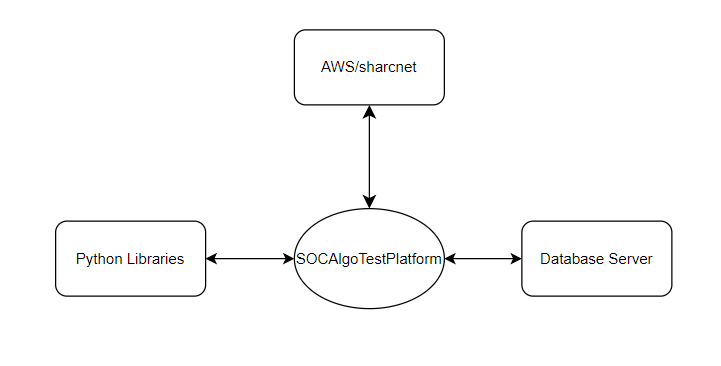
\includegraphics[width=1\linewidth]{diagrams/partner_applications.png}
\end{figure}
\subsection{Off-the-Shelf Software}

\begin{table}[H]
    \centering
    \begin{tabular}{|1|1|}
         \hline \textbf{Partner Application} & \textbf{Usage} \\
         \hline Matlab & compile/execute user-provided algorithms \\
         \hline Database Server & Persist necessary data \\
         \hline Various python libraries & Open-source libraries will be used for providing standard \\
         & functionality (i.e. an SQL driver, web server framework)\\
         \hline
    \end{tabular}
\end{table}
\subsection{Anticipated Workplace Environment}
As the product is a web application it will be used in any environment that has an internet connection. 
\subsection{Schedule Constraints}
\begin{itemize}
    \item Problem Statement, POC Plan, Development Plan - Sep 16
    \item Requirements Document Revision 0 - Oct 11
    \item Hazard Analysis 0 -Oct 23
    \item V\&V Plan Revision 0 - Nov 1
    \item POC Demo - Nov 11-22
    \item Design Document Revision 0 - Jan 15
    \item Revision 0 Demo - Feb 3
    \item V\&V Report Revision 0 - Mar 7
    \item Final Demo Rev 1 - March 24
    \item EXPO Demo - April
    \item Final Doc - Apr 2
\end{itemize}
\subsection{Budget Constraints}
The budget to create the project is \$750 coming from the team. No hard budget exists to run the system, but a strong emphasis is placed on having the lowest possible operational costs for the running system.
\subsection{Enterprise Constraints}
N/A. (As this is an academic project, there is no “Enterprise” sponsoring the project providing additional constraints.)

\section{Naming Conventions and Terminology}
\subsection{Glossary of All Terms, Including Acronyms, Used by Stakeholders
involved in the Project}
\begin{itemize}
\item SOC - State of charge
\item AWS - amazon web service
\item Leaderboard - a table displaying the results of all algorithms submitted by all users with categories that can be filtered on/sorted. 
\item Algorithm - algorithms submitted by users to be tested for efficiency and performance.
\item Performance - quantitative measurement of the algorithm’s performance in different categories

\end{itemize}



\section{Relevant Facts And Assumptions}
\subsection{Relevant Facts}
\begin{itemize}
\item Running tests on an algorithm typically takes about an hour to complete.
\item The existing application is only capable of executing tests in serial, no support exists for parallel test execution.
\item The current application supports executing Matlab algorithms only.
\item Responses from the current application are handled via email.
\end{itemize}
\subsection{Business Rules}
\begin{itemize}
    \item The system must not have excessive hosting costs
\end{itemize}
\subsection{Assumptions}
\begin{itemize}
    \item Applicable Matlab licensing is available and affordable.
	\item Required Cloud resources are available and affordable.
\end{itemize}

\section{The Scope of the Work}
\subsection{The Current Situation}
\begin{figure}[H]
    \centering
    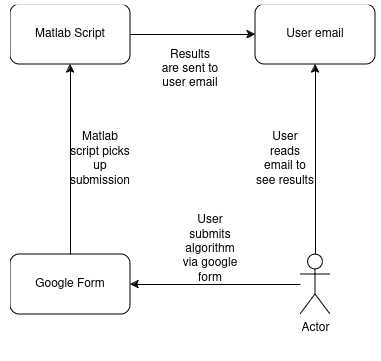
\includegraphics[width=1\linewidth]{diagrams/currentstate.png}
\end{figure}

\subsection{The Context of the Work}
\begin{figure}[H]
    \centering
    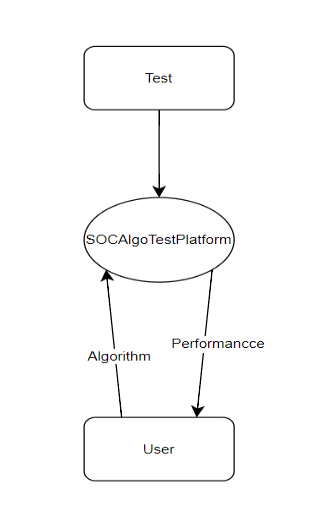
\includegraphics[width=0.5\linewidth]{diagrams/context.png}
\end{figure}
\subsection{Work Partitioning}

\begin{table}[H]
    \centering
    \begin{tabular}{| 1 | 1 | 1 | 1 |}
    \hline
         Business Event Number & Business Event Name & Input and Output & Summary of BUC \\
    \hline
         1 & User & User email and & Process user \\
         & registration/Login & password (in) & registration \\
        \hline
         2 & Submission of & File with an & Process algorithm \\
          & algorithm & algorithm (in) & submission and \\
          & & & initiate testing \\
         \hline
         3 & Completion of & Results of algorithm & Generate and store \\
         3 & algorithm testing & performance (out) & the results of \\
         & & & algorithm \\
         & & & performance \\
         \hline
         4 & Leaderboard & Results of algorithm & Update the \\
          & Update & performance (in) & leaderboard to \\
          & & Update leaderboard & allow performance \\
          & & (out) & comparison\\
 \hline
    \end{tabular}
\end{table}


\subsection{Specifying a Business Use Case (BUC)}
Scenario 1: Process user registration/Login \\
	Actor: user \\
	Precondition: N/A \\
	Trigger: user clicks sign up \\
	Steps: \\
User accesses the registration page and submit his email, name, institution and password
System does some validation and create the account \\
User can now login using his/her credentials \\
	Postcondition: New user is added to DB \\

	Scenario 2: Submission of algorithm \\
	Actor: user \\
	Precondition: User is logged into his account \\
	Trigger: user submits an algorithm \\
	Steps: \\
User accesses the algorithm submission page and upload his/her algorithm file. \\
System validates submission and display success/failure to upload \\
System displays the status of the test \\
	Postcondition: Algorithm is being tested \\

Scenario 3: Completion of algorithm testing \\
Actor: system \\
	Precondition: An algorithm was submitted and is being tested \\
	Trigger: algorithm testing is complete \\
	Steps: \\
System calculates and reports the performance of the algorithm \\
System notifies the user if the testing is done/if any errors was encountered \\
	Postcondition: performance results are stored in db that can be accessed by user \\

Scenario 4: Leaderboard update \\
Actor: system \\
	Precondition: An algorithm was tested successfully \\
	Trigger: algorithm testing is complete \\
	Steps: \\
System receives the new algorithm results and updates the leaderboard table in the database. \\
	Postcondition: Leaderboard is up to date \\


\section{Business Data Model and Data Dictionary}
\subsection{Business Data Model}
\begin{figure}[H]
    \centering
    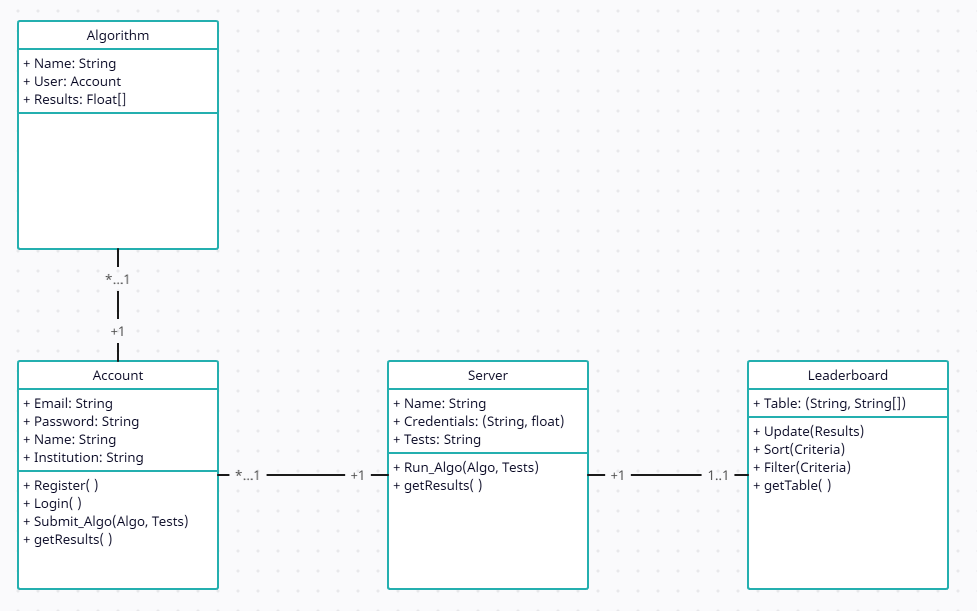
\includegraphics[width=1\linewidth]{diagrams/Class.png}
\end{figure}
\subsection{Data Dictionary}
\begin{table}[H]
    \centering
    \begin{tabular}{|1|1|1|}
         \hline \textbf{Name} & \textbf{Content} & \textbf{Type} \\
         \hline Account & Email + Name + Institution + Password & Class \\
         \hline Leaderboard & Compilation of Performances & Class \\
         \hline Algorithm & Results and files & Class \\
         \hline Email & “”@””.”” & Class \\
         \hline Name & String & Attribute/Element \\
         \hline Institution & String & Attribute/Element \\
         \hline Password & String & Attribute/Element \\
         \hline Algorithm Name & String & Attribute/Element \\
         \hline User & Account & Attribute/Element \\
         \hline Results & Float[] & Attribute/Element \\
         \hline Server Name & String & Attribute/Element \\
         \hline Credentials & (String, Float) & Attribute/Element \\
         \hline Tests & String (Name of the script containing tests) & Attribute/Element \\
         \hline
    \end{tabular}
\end{table}

\section{The Scope of the Product}
\subsection{Product Boundary}
\begin{figure}[H]
    \centering
    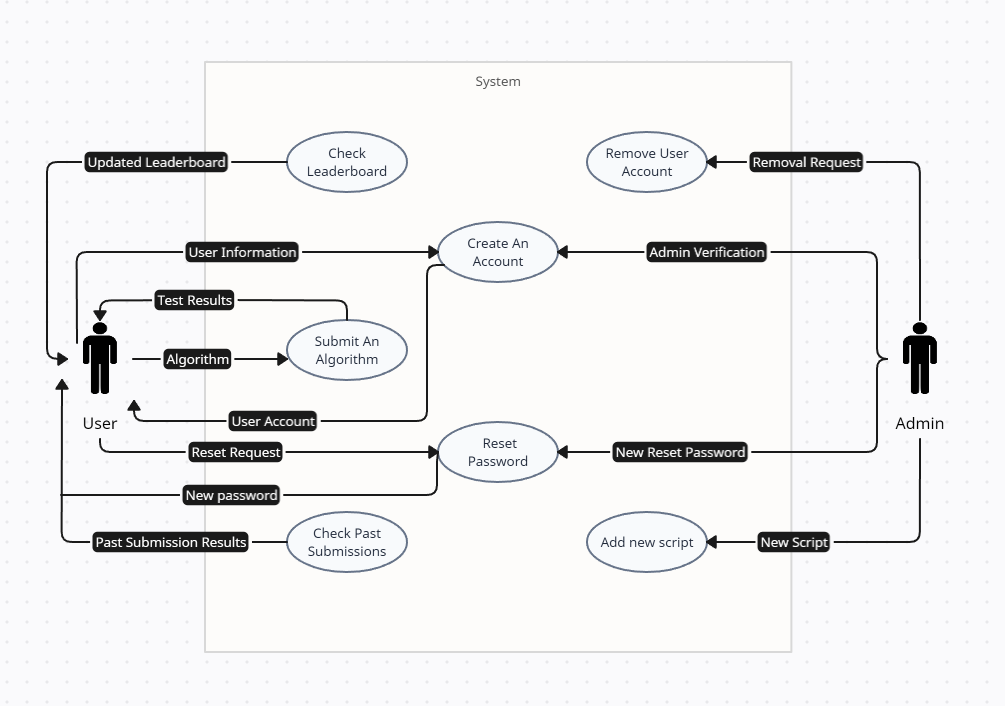
\includegraphics[width=1\linewidth]{diagrams/Use.png}
\end{figure}
\subsection{Product Use Case Table}
\begin{table}[H]
    \centering
    \begin{tabular}{|1|1|1|1|}
         \hline \textbf{PUC No} & \textbf{PUC Name} & \textbf{Actor/s} & \textbf{Inputs \& Outputs}\\
         \hline 1 & Submit An Algorithm & User & Algorithm (In), \\
         & & & Test results (Out)\\
         \hline 2 & Check Leaderboard & User & Updated Leaderboard (Out)\\
         \hline 3 & Check Past Submissions & User & Past submissions (Out)\\
         \hline 4 & Create An Account & User, Administrator & User information (In), \\
         & & & Admin Verification (In), \\
         & & & User Account (Out)\\
         \hline 5 & Reset Password & User, Administrator & Reset Request (In), \\
         & & & Reset Password (In), \\
         & & & New password (Out)\\
         \hline 6 & Remove User Account & Administrator & Removal Request (In)\\
         \hline 7 & Add New Script & Administrator & New script (In)\\
         \hline
    \end{tabular}
\end{table}
\subsection{Individual Product Use Cases (PUC's)}
\begin{enumerate}
    \item A user creates a battery testing algorithm and wants it to be tested to see how efficient it is. They submit the algorithm to the system and after the system has completed the tests, it outputs the results back to the user.
    \item A user navigates to the leaderboard screen to check what the current best algorithm for testing batteries is and which user created it. The system outputs the updated leaderboard results to the user.
    \item A user navigates to their account page and wants to view the results of all algorithms they have submitted previously. The system will display these previous submissions to the user.
    \item A user navigates to the main page of the website and inputs their information. The system inputs this system and requests an administrator reviews the information for correctness. Once the administrator has verified the information, the system will create the account for the user.
    \item A user forgets their password and sends a request to the system to reset it. An administrator creates a new temporary password for the user and sets the users current password to this temporary one. The system notifies the user of this new password.
    \item An administrator wants to delete a user account for violating terms of service. They submit a request to the system to delete this user account and the system ensures it is deleted.
    \item An administrator discovers new tests that they want to include within the script that the system runs against user algorithms. The administrator uploads this new script within the system and the system now runs the new script.
\end{enumerate}


\section{Functional Requirements}
\subsection{Functional Requirements}
\textbf{FR-1}
\begin{itemize}
    \item The system shall allow users to submit algorithms to be tested. \hfill \break
    Fit criterion: Users should be able to upload an algorithm to the system and receive confirmation of their upload.
\end{itemize}
\textbf{FR-2}
\begin{itemize}
    \item The system shall report the results of submitted algorithms when their testing is complete. \hfill \break
    Fit criterion: Users should be able to view the result of their algorithm somewhere in the interface of the system after it has been completed.
    \break
    Depends on: FR-1
\end{itemize}
\textbf{FR-3}
\begin{itemize}
    \item The system shall allow for multiple submissions from users to run in parallel. \hfill \break
    Fit criterion: Users should be able to submit more than one algorithm for testing and see that the execution of all submissions is underway.
    \break
    Depends on: FR-1
\end{itemize}
\textbf{FR-4}

\begin{itemize}
    \item The system shall allow users to make a new account. \hfill \break
    Fit criterion: Users should be able to provide a username and password and in return gain access to a new account corresponding to those values.
\end{itemize}
\textbf{FR-5}
\begin{itemize}
    \item The system shall have a user login page. \hfill \break
    Fit criterion: Users should be able to navigate to a page in the system where they can provide a username and password to authenticate under an account.
\end{itemize}
\textbf{FR-6}
\begin{itemize}
    \item The system shall segregate data based on the logged users. \hfill \break
    Fit criterion: Users should not be able to see the private data of users and vice versa. \\
    Depends on: FR-4
\end{itemize}
\textbf{FR-7}
\begin{itemize}
    \item The system shall save algorithm results in individual user accounts. \hfill \break
    Fit criterion: Users should be able to view their previous submissions anytime in the future. \\
    Depends on: FR-4
\end{itemize}
\textbf{FR-8}
\begin{itemize}
    \item The system shall have a leaderboard feature that is accessible to all users. \hfill \break
    Fit criterion: Users should be able to view a list of all submissions from other users.
\end{itemize}
\textbf{FR-9}
\begin{itemize}
    \item The system shall have categorization in its leaderboard based on certain criteria. \hfill \break
    Fit criterion: Users should be able to select the type of algorithm they are interested in and only view results of that type. \\
    Depends on: FR-8
\end{itemize}
\textbf{FR-10}
\begin{itemize}
    \item The system shall allow users to sort through the leaderboards based on criteria. \hfill \break
    Fit criterion: Users should be able to view results in order of lowest run time to highest or other criteria. \\
    Depends on: FR-8
\end{itemize}
\textbf{FR-11}
\begin{itemize}
    \item The system shall display the progress of running algorithms to users. \hfill \break
    Fit criterion: Users should be able to view if a submission is accepted, pending, executed, or finished.
\end{itemize}
\textbf{FR-12}
\begin{itemize}
    \item The system shall notify users in case of an exception in their algorithm. \hfill \break
    Fit criterion: Users should receive a notification if their algorithm fails to execute successfully.
\end{itemize}

\section{Look and Feel Requirements}
\subsection{Appearance Requirements}
\textbf{LFR-1}
\begin{itemize}
    \item The system’s appearance should look similar to a website called Kaggle. \hfill \break
    Fit criterion: Users should recognize similarities between the system and Kaggle.
\end{itemize}

\subsection{Style Requirements}
\textbf{SR-1}
\begin{itemize}
    \item The system should use the same styles i.e. colour, background colour, user-interface structure, etc. as the Kaggle website. \hfill \break
    Fit criterion: Users should see the same styles as the Kaggle website when using the system.
\end{itemize}


\section{Usability and Humanity Requirements}
\subsection{Ease of Use Requirements}
\textbf{EUR-1}
\begin{itemize}
    \item All tasks that can be completed with the system should have a similar workflow.\hfill \break
    Fit criterion: Users should be able to follow the same workflow when viewing a submission in progress or one that is already completed.
\end{itemize}
\subsection{Personalization and Internationalization Requirements}
N/A - No personalization or internationalization was mentioned by the client.
\subsection{Learning Requirements}
\textbf{LR-1}
\begin{itemize}
    \item The system shall have detailed documentation for all core functionality. \hfill \break
    Fit criterion: Users should be able to easily find documentation which walks them through the steps involved in submitting an algorithm and viewing the results.
\end{itemize}
\textbf{LR-2}
\begin{itemize}
    \item The system shall display hints for new/unused features for a specific user. \hfill \break
    Fit criterion: The user should be able to see a hint indicating how to use a new feature.
\end{itemize}

\subsection{Understandability and Politeness Requirements}
\textbf{UPR-1}
\begin{itemize}
    \item The system shall use universally used symbols when appropriate to ease understanding. \\
    Fit criterion: At least 90\% of users should be able to correctly identify the meaning of all symbols without explanation. 
\end{itemize}
\textbf{UPR-2}
\begin{itemize}
    \item The system shall use an intuitive user interface and use consistent terminology. \\
    Fit criterion: The terminology used on each page should be consistent with each other and at least 80\% of users should be able to navigate through each stage of the system without external assistance. 
\end{itemize}
\textbf{UPR-3}
\begin{itemize}
    \item The system shall provide visual feedback to indicate whether certain actions were successful or not.
\end{itemize}
\textbf{UPR-4}
\begin{itemize}
    \item The system shall provide walkthroughs for any complex use cases.
\end{itemize}

\subsection{Accessibility Requirements}
\textbf{AR-1}
\begin{itemize}
    \item The system shall have a colour-blind mode
\end{itemize}

\section{Performance Requirements}
\subsection{Speed and Latency Requirements}
\textbf{SLR-1}
\begin{itemize}
\item The product shall display the results of algorithms in less than 2 seconds after it is requested \hfill \break
Fit Criteria: Users should see a result after selecting an algorithm to view in under 2 seconds
\end{itemize}
\textbf{SLR-2}
\begin{itemize}
\item The product shall display the Leaderboards table in less than 3 seconds after it is requested \hfill \break
Fit Criteria: Users should see the leaderboards after selecting that view in under 3 seconds
\end{itemize}
\textbf{SLR-3}
\begin{itemize}
\item Sorting or filtering the leaderboard should not take more than 3 seconds \hfill \break
Fit Criteria: Users should see leaderboard content change in under 3 seconds after making a change to filtering criteria
\end{itemize}


\subsection{Safety-Critical Requirements}
N/A - we are building a web application without any interaction with the physical world
\subsection{Precision or Accuracy Requirements}
\textbf{PAR-1}
\begin{itemize}
    \item Events in the system will be tracked using standard UTC timestamp
\end{itemize}
\subsection{Robustness or Fault-Tolerance Requirements}
\textbf{RR-1}
\begin{itemize}
    \item The system should be able to handle any types of errors during run-time.
\end{itemize}
\textbf{RR-2}
\begin{itemize}
    \item Errors arising from one users interactions with the system should be isolated from other users interactions
\end{itemize}

\subsection{Capacity Requirements}
\textbf{CR-1}
\begin{itemize}
    \item The system shall support concurrent requests from a few hundred users \hfill \break
    Fit criterion: Users should not see a difference in performance when there is one current user or one hundred current users.
\end{itemize}

\subsection{Scalability or Extensibility Requirements}
\textbf{SR-1}
\begin{itemize}
    \item The system shall automatically scale its execution backend corresponding to the number of user requests
\end{itemize}

\subsection{Longevity Requirements}
\textbf{LR-1}
\begin{itemize}
    \item The system shall be free of memory leaks and uncapped caches so that restarts will not be required
\end{itemize}

\section{Operational and Environmental Requirements}
\subsection{Expected Physical Environment}
N/A - The product shall work in any environment with an internet connection.

\subsection{Wider Environment Requirements}

\textbf{WER-1}
\begin{itemize}
    \item The system shall adhere to the best practices in data privacy to protect user information \hfill \break
    Fit criterion: The system shall have secure login methods and keep any data from being accessed externally.
\end{itemize}

\subsection{Productization Requirements}
\textbf{PR-1}
\begin{itemize}
    \item The product shall be deployable on AWS and accessible to the users through the web.
\end{itemize}

\subsection{Release Requirements}
N/A - there will not be regular releases for this project, and maintenance will be done by an external team.

\section{Maintainability and Support Requirements}
\subsection{Maintenance Requirements}
\textbf{MR-1}
\begin{itemize}
    \item If a likely change is made to the finished software, it will take at most 10\% of the original development time, assuming the same development resources are available (Example from a lecture that Dr. Smith said we can use if we do not think of anything else)
\end{itemize}
\subsection{Supportability Requirements}
\textbf{SUR-1}
The product must be self-supporting with all the necessary information provided in the user documentation and/or user guides.

\subsection{Adaptability Requirements}
\textbf{ADR-1}
\begin{itemize}
    \item The product shall work under all major operating systems such as macOS, Linux and Windows. \hfill \break
    Fit criterion: Users should be able to access the system and its functionality on any of the above-listed operating systems.
\end{itemize}
\textbf{ADR-2}
\begin{itemize}
    \item The product shall be compatible with all major browsers like Chrome, Safari, Microsoft Edge, Opera, and Firefox. \hfill \break
    Fit criterion: Users should be able to access the system and its functionality on any of the above browsers.
\end{itemize}


\section{Security Requirements}
\subsection{Access Requirements}
\textbf{ACR-1}
\begin{itemize}
    \item The system shall verify the credentials passed onto the login screen before giving access to the system. \hfill \break
    Fit criterion: A valid email and password combination should be passed in by the user before the user can access the system.
\end{itemize}
\textbf{ACR-2}
\begin{itemize}
    \item The system shall allow only verified users to view information about other accounts. \hfill \break
    Fit criterion: Non-logged-in users should not be able to view information about other users.
\end{itemize}
\textbf{ACR-3}
\begin{itemize}
    \item The system shall allow only administrators to see the emails of users. \hfill \break
    Fit criterion: Non-admin users should not have access to the emails of other users.
\end{itemize}

\subsection{Integrity Requirements}
\textbf{IR-1}
\begin{itemize}
    \item The database shall prevent incorrect data from being introduced.
\end{itemize}
\textbf{IR-2}
\begin{itemize}
    \item The database shall be regularly backed up in case of any failure
\end{itemize}

\subsection{Privacy Requirements}
\textbf{PRR-1}
\begin{itemize}
    \item The product shall collect, store and use the user’s email address for the login verification process only.
\end{itemize}
\textbf{PRR-2}
\begin{itemize}
    \item The product shall not share its users’ email addresses with third parties under any circumstance. 
\end{itemize}
\subsection{Audit Requirements}
N/A - The use of the product will not involve any sensitive data. It will also not be subject to any government regulations so auditing requirements are not needed.

\subsection{Immunity Requirements}
\textbf{IR-1}
\begin{itemize}
    \item The product shall ensure that only verified users are allowed to submit algorithms
\end{itemize}
\textbf{IR-2}
\begin{itemize}
    \item The product shall ensure that user-submitted algorithms are executed in a secure and isolated environment and prevent malicious actions.
\end{itemize}

\section{Cultural Requirements}
\subsection{Cultural Requirements}
\textbf{CUR-1}
\begin{itemize}
    \item The product shall not be offensive to any group of people.
\end{itemize}

\section{Compliance Requirements}
\textbf{LGR-1}
\subsection{Legal Requirements}
\begin{itemize}
    \item In compliance with the Matlab End-user license agreement. \hfill \break
    Fit criterion: The system must adhere to the licensing terms and conditions in the Matlab EULA.

\end{itemize}
\subsection{Standards Compliance Requirements}
\textbf{SCR-1}
\begin{itemize}
    \item General Data Protection Regulation compliance should be the target for user data. \hfill \break
    Fit criteria: The system must ensure only necessary data are collected from users and that the data are processed and stored per GDPR. 

\end{itemize}

\section{Open Issues}
\begin{itemize}
    \item Investigate Matlab licensing and the integration of Matlab submissions with our system.
    \item Explore different AWS pricing
\end{itemize}

\section{Off-the-Shelf Solutions}
\subsection{Ready-Made Products}
N/A - This system is a rebuild of an existing application (Borealis), for which there are no existing solutions on the market.
\subsection{Reusable Components}
\begin{itemize}
    \item REACT
    \item AWS
\end{itemize}

\subsection{Products That Can Be Copied}
\begin{itemize}
    \item Kaggle: The format of Kaggle fits our use case well, with the difference being the type of algorithms being evaluated. Kaggle can be used as a guide for how the front end of the service should function.
\end{itemize}

\section{New Problems}
\subsection{Effects on the Current Environment}
Since this is a completely new system, users will have to adapt and learn how to use it and potentially change their workflow. 
\subsection{Effects on the Installed Systems}
\begin{itemize}
    \item In this case, while some software will be reused from the existing system, the new system is intended to replace the existing system, so they will not interact. The old system will be decommissioned after the new system is deployed.
\end{itemize}

\subsection{Potential User Problems}
It is possible that performance and scaling issues could arise while using the system which could cause users to get frustrated with the system. It is also possible that the submitted algorithms might not work with the system due to different versioning/ if the system is implemented in GnuOctave instead of Matlab and certain libraries or methods fails to work. Other potential issues could be problems with usability and security. To mitigate these concerns, regular feedback from stakeholders should be taken. Also, sufficient performance and security testing will be needed.

\subsection{Limitations in the Anticipated Implementation Environment That May
Inhibit the New Product}
\begin{itemize}
    \item Use of Matlab; we need to either run many concurrent instances of a Matlab interpreter or efficiently compile Matlab code repeatedly to execute user submissions. We may encounter issues with either licensing or product performance here
    \item Cloud Costs: Using AWS for hosting the execution backend may be prohibitively expensive
\end{itemize}

\subsection{Follow-Up Problems}
\begin{itemize}
    \item In the event the product achieves widespread use, the cost of computing may be too high to support the product with a large number of users (1000s of concurrent users)
\end{itemize}

\section{Tasks}
\subsection{Project Planning}
\textbf{Task List:}
\begin{itemize}
    \item Problem Description (Required by September 23, 2024)
    \item SRS document (Required by October 9, 2024)
    \item Hazard Analysis (Required by October 23, 2024)
    \item VnV plan (Required by November 1, 2024)
    \item Create Django Framework (Required by November 11, 2024)
    \item Configure Submissions Within Django Framework (Required by November 11, 2024)
    \item Configure Leaderboard Feature Within Django Framework (Required by November 11, 2024)
    \item Configure User Accounts and Registration Within Django Framework (Required by November 11, 2024)
    \item POC (Required by November 11, 2024)
    \item Design Document (Required by January 15, 2025)
    \item Design to Look Similar to Kaggle (Required by February 3, 2025)
    \item Product Revision 0 (Required by February 3, 2025)
    \item VnV Report (Required by March 7, 2025)
    \item Create Tutorial Videos (Required by April 2, 2025)
    \item Final Revision (Required by April 2, 2025)
\end{itemize}

\subsection{Planning of the Development Phases}
\begin{itemize}
\item Proof of Concept stage:
This stage aims to provide the basic functionality of the new system, accept an algorithm submission, run it against the existing test script, and report the results back to the user. This stage must be operational by November 11th, 2024. The operational environment components involved are the hosting provider used for the front end, as well as the hosting provider used for the back end (these may not necessarily be the same). The function requirements involved at this stage are
\begin{itemize}
    \item The system shall allow users to submit algorithms to be tested 
\item The system shall report the results of submitted algorithms when their testing is complete
\item The system shall allow for multiple submissions from users to run in parallel. 
\end{itemize}

None of the non-functional requirements are in scope at this stage

\item Revision 0 stage:
This stage aims to provide the first working version of the system with complete functionality. This stage must be complete by February 3rd, 2025. All operational environment components are involved, as are all functional and non-functional requirements
	
\item Revision 1 stage:
This stage aims to provide an improved complete version of the system, based on the learnings from the development and testing of revision 0. This stage must be completed by March 17th, 2024. Once again all operational environment components are involved, as are all requirements. Additional requirements not discovered before the revision 0 stage may enter the scope here and be included in this development phase.  
\end{itemize}


\section{Migration to the New Product}
\subsection{Requirements for Migration to the New Product}
N/A - The existing system had no accounts/history or storage of results since results were emailed directly to users.

\subsection{Data That Has to be Modified or Translated for the New System}
N/A - Existing results of previously submitted algorithms can be discarded once users switch to the new system.

\section{Costs}
\begin{itemize}
    \item During the development and testing phase, the application will not be under heavy load so cloud hosting costs should be less than \$100
\end{itemize}

\section{User Documentation and Training}
\subsection{User Documentation Requirements}
As part of user documentation, the software will come with a user guide as well as walkthroughs that are built into the application, similar to how GitHub presents its tutorials.

\subsection{Training Requirements}
\begin{itemize}
    \item Hints will be provided for new functionality to help board new users
    \item Video explanations can be added for complex components of the application
\end{itemize}

\section{Waiting Room}
\begin{itemize}
    \item Submit algorithms in a variety of other programming languages (not exclusively accepting matlab algorithms)
\end{itemize}

\section{Ideas for Solution}
\begin{itemize}
    \item SHARCNET
    \item AWS ECS
    \item AWS MATLAB prebuilt machine image
\end{itemize}


\newpage{}
\section*{Appendix --- Reflection}

The information in this section will be used to evaluate the team members on the
graduate attribute of Lifelong Learning.  Please answer the following questions:

\begin{enumerate}
  \item What knowledge and skills will the team collectively need to acquire to
  successfully complete this capstone project?  Examples of possible knowledge
  to acquire include domain-specific knowledge from the domain of your
  application, software engineering knowledge, mechatronics knowledge or
  computer science knowledge.  Skills may be related to technology, or writing,
  or presentation, team management, etc.  You should look to identify at
  least one item for each team member.
  \item For each of the knowledge areas and skills identified in the previous
  question, what are at least two approaches to acquiring the knowledge or
  mastering the skill?  Of the identified approaches, which will each team
  member pursue, and why did they make this choice?
\end{enumerate}

\begin{enumerate}
  \item \textbf{Nathan Uy}
\begin{itemize}
    \item Being a team player is crucial to completing this project. Effective communication skills are necessary to manage conflicts and convey priorities and expectations from one another. Planning effectively, adapting to change, and problem-solving will also be needed throughout the project development since there will be changes in the requirements, tight deadlines and other unexpected changes that the team should be prepared for.
\end{itemize} 
\textbf{Declan Young}
\begin{itemize}
    \item Developing knowledge of best practices for both frontend and backend development to ensure that the two work together seamlessly is another critical aspect of the success of this capstone project. Since there are multiple components that must work together in order for the application being developed to function efficiently and effectively, it will be important to ensure that each performs as expected individually, but also when iterating with each other. 
\end{itemize} 
\textbf{Benjamin Dubois}
\begin{itemize}
    \item Knowledge of configuring and maintaining a server will be crucial for our success in this capstone project. For this project, we will be developing a server that will allow for submissions to be tested in parallel and the majority of our project depends on this being successful as this is the number one requirement of our stakeholders.
\end{itemize}
\textbf{Aidan Mariglia}
\begin{itemize}
    \item Success for this project hinges on our ability to manage many concurrently executing backend jobs, ensuring that throughput is high enough to provide a smooth experience to our users, while not producing high hosting costs. Managing a many concurrent job is a frequent task in backend engineering, so the skill most important to the success of this project is backend design.
\end{itemize}
\item \textbf{Team Working skills}
\begin{itemize}
\item Experience working in a team will help us acquire great communication skills, project management skills and conflict management skills. Participating in team-building activities or any hands-on team activities can also strengthen these skills. We will ensure to continually engage within our group to enhance our communication skills and project management skills and do retrospectives on how we could improve next time.
\end{itemize}
\textbf{Best practices for both frontend and backend}
\begin{itemize}
    \item The first approach that can be used is referencing documentation, textbooks, research or other references on best practices to ensure that both the frontend and backend are developed properly. Additionally, using this information will allow our group to acquire a significant amount of knowledge and skills regarding these topics, which will allow us to make more informed decisions on less standard topics and issues related to these fields that we are encountering throughout the duration of the project.
    \item Another approach is experimenting with different technologies to see how different frontend and backend frameworks and technologies interact with each other. This will give us examples of different approaches to frontend and backend development, which we can apply to each iteration of the project.
\end{itemize}
\textbf{Knowledge of configuring and maintaining a server}
\begin{itemize}
\item The first approach to gaining this knowledge can be working on a test system and experimenting with features to ensure we know what works well and what we need to improve on. This can be considered the trial and error approach as if we make any changes on this test server that cause major issues, it is not a problem.
\item Another approach that can be used is referencing online tutorials and walkthroughs from experts in this field. There are millions of videos available that can be very helpful in gaining this knowledge. This is the approach that our team is going to pursue as it is more efficient than trial and error and does not require the setup of a test server. 
\end{itemize}
\textbf{Backend Design}
\begin{itemize}
\item The first approach to gaining this knowledge is studying theory. Many resources exist which discuss design patterns and other techniques which aid in efficient backend design. Studying these techniques provides a developer with the necessary background knowledge to make the correct design decisions.
\item The second approach to gaining backend design knowledge is experience. Through designing many systems, and making mistakes, an intuitive knowledge is gained for backend design methodology, making future decisions easier and previous mistakes avoidable. This is the approach which will be used by the team, in order to leverage our existing co-op work experience.
\end{itemize}

\end{enumerate}

\end{document}